\documentclass[12pt,oneside,a4paper]{article}   
\usepackage[czech, english]{babel}
\usepackage{amsmath}
%\usepackage{epsf,epic,eepic,eepicemu,url,graphicx}
\usepackage{epsf,url,graphicx}
\usepackage[utf8]{inputenc}
\usepackage{float}
\usepackage{todonotes}
\usepackage{listings}
\usepackage{caption}

%% code listings, pretty simple, but works quite ok :-)
\newenvironment{listing}
{\begin{list}{}{\setlength{\leftmargin}{1em}}\item\scriptsize\bfseries}
{\end{list}}

\definecolor{light-gray}{gray}{0.65}

\DeclareCaptionFont{white}{\color{white}}
\DeclareCaptionFormat{listing}{\colorbox{light-gray}{\parbox{\textwidth}{#1#2#3}}}
\captionsetup[lstlisting]{format=listing,labelfont=white,textfont=white}

\lstset{
	basicstyle=\footnotesize\ttfamily,
	numberstyle=\tiny,
	numbersep=5pt,
	tabsize=2,
	extendedchars=true,
	breaklines=true,
	%	showstringspaces=true,
	keywordstyle=\color{red},
	frame=b,         
	stringstyle=\color{white}\ttfamily,
	showspaces=false, 
	showtabs=false,  
	xleftmargin=17pt,
	framexleftmargin=17pt,
	framexrightmargin=5pt,
	framexbottommargin=4pt,
	showstringspaces=false, 
	breakatwhitespace=true,
	commentstyle=\color{pgreen},
	keywordstyle=\color{pblue},
	stringstyle=\color{pred}    
}
\lstloadlanguages{Java}

\begin{document}
\begin{center}
\bf MI-VMW\\[2mm]
    \begin{Large}Flickr - re-ranking založený na metadatech\end{Large}\\[3mm]
       Michal Sláma (slamamic@fit.cvut.cz)\\
       Šimon Steklík (steklsim@fit.cvut.cz)\\
leden 2016
\end{center}

\section{Zadání}
Cílem projektu je vytvoření aplikace umožňující vylepšené vyhledávání ve fotografiích uložených na serveru
Flickr. Flickr poskytuje aplikační rozhraní umožňující získat prakticky libovolná data o fotografiích, která jsou
přístupna i z oficiálního webového rozhraní. Cílem projektu je tedy aplikace, která umožní vyhledávání na
flickru založené na klíčových slovech, stejně jako je tomu na Flickru nyní, ale navíc bude možné zadat
sekundární vyhledávání na libovolná metadata.

\subsection{Vstupy}
Klíčové slovo, sada hodnot metadat pro setřídění a počet výsledků (omezení velikosti výstupu).
Jako metadata určená k rerankingu jsme zvolili tato:
\begin{itemize}
	\item Řetězec - popis obrázku.
	\item GPS - místo kde byla fotka pořízena.
	\item Integer - počet zhlédnutí obrázku.
	\item Datum - datum pořízení obrázku.
\end{itemize}
U každého z metadat bude možné zvolit jeho váhu (míru důležitosti).

\subsection{Výstup}
Fotky, jejichž popis odpovídá klíčovému slovu. Fotky budou setříděné podle vzdálenosti ke zvoleným
metadatům.

\section{Způsob řešení}
V této sekci je popsán použitý způsob rerankingu obecně a pro jednotlivé typy metadat.

\subsection{Obecné principy}
Reranking se dá obecně popsat jako "znovuseřazení" nějaké už řazené množiny -- v našem případě je první fází vyhledání fotek na Flickeru podle klíčového slova a množina výsledků tohoto hledání je poté seřazena podle "vzdálenosti" k použitým metadatům. Tato vzdálenost se pro různé typy dat počítá rozdílně a existuje mnoho způsobů jejího výpočtu; ve druhé části této kapitoly budou popsány námi vybrané typy výpočtu pro jednotlivé typy metadat.

Tyto vzdálenosti je pak třeba zkombinovat do jedné hodnoty, podle které jsou pak obrázky seřazeny -- toto bude popsáno na konci kapitoly.

\subsection{Typy metadat}
\subsubsection{Řetězec}
Pro výpočet vzdálenosti mezi řetězci jsme zvolili \textit{Levenstheinovu vzdálenost}, která definuje vzdálenost jako počet přidání, odebrání a nahrazení písmen potřebných pro transformaci jednoho řetězce na druhý \cite{Levensthein}.
Např. řetězce \texttt{"rank"} a \texttt{"tank"} mají vzdálenost 1 (výměna "r" za "t"), \texttt{"rank"} a \texttt{"rerank"} jsou ve vzdálenosti 2.

Při implementaci je využito dynamického programování, protože naivní rekurzivní algoritmus si v rozumném čase neporadí s řetězci delšími než cca 10 znaků \cite{Levensthein_java}.

\subsubsection{GPS}
Při výpočtu vzdálenosti mezi dvěma body na zeměkouli (bod kde byla fotografie pořízena a bod vybraný uživatelem) jsme použili \textit{Great-circle Distance}, která počítá vzdálenost dvou bodů na povrchu (ideální) koule \cite{GCD}. Není tedy na Zemi úplně přesná, ale pro naše účely plně postačuje.

\subsubsection{Datum}
Vzdálenost mezi daty (datum pořízení fotografie a datum vybrané uživatelem) počítáme jednoduše jako absolutní hodnotu jejich rozdílu ve dnech.

\subsubsection{Celá čísla}
Vzdálenost mezi celými čísly (počet zklédnutí fotografie a číslo určené uživatelem) počítáme jednoduše jako absolutní hodnotu jejich rozdílu.

\subsection{Kombinace vzdáleností (normalizace, decay funkce)}
Rozsah hodnot jednotlivých typů metadat není stejný (u některých teoreticky neomezený). Mohlo by se tedy stát, že fotografie, která se shoduje ve všech metadatech kromě jednoho, kde je rozdíl hodnot naopak obrovský, bude nesprávně upozaděna oproti fotografii, která se liší ve všech metadatech, ale v řádově menší míře. Je proto třeba vzdálenosti nějakým způsobem \textit{normalizovat} -- převést do určitého společného rozsahu hodnot.

My pro převedení do rozsahu \textit{(0, 1)} používáme tuto \textit{decay funkci}:
\begin{equation}
	f(x) = 1 - e^{-\lambda x}
\end{equation}
kde \(x\) je vypočtená vzdálenost a \(\lambda\) je parametr určující rychlost růstu funkce (čím větší je \(\lambda\), tím rychleji hodnota funkce roste k jedničce). Pro každý typ metadat je \(\lambda\) nastavena jinak (podle předpokládaného rozsahu hodnot daných metadat).

Celkový \textit{rank} (menší je lepší) každé fotografie je pak dán součtem hodnot u všech typů metadat.

\subsection{Váhy metadat}
Uživatel má možnost u každého typu metadat určit, jakou váhu mu přisuzuje -- výsledky s nízkou vzdáleností u daného typu budou pak upřednostněny více nebo méně. Pro naše účely jsme zvolili jednoduchou volbu z 5 hodnot (vah): 0, 0.5, 1, 1.5, 2 (0 ve výsledku vypne řazení podle daného typu metadat).

\section{Implementace}

\subsection{Java}

Aplikace je implementována v programovacích jazyce Java s využitím frameworku Spring s architekturou MVC (Model-View-Controller).
Front-end je pak realizován pomocí jsp a využívá css a javascript od boostrapu a jquery.

Vypíchnout můžeme způsob stažení a rerankingu fotek z flickru. Stažení a reranking je realizováno v samostatných vláknech na principu producent/ konzument. Fotky jsou z flickru staženy vždy po stránkách jejichž velikost je konfigurovatelná pomocí property souboru. Stažené fotky jsou umístěny do sdíleného uložiště mezi oběma vlákny. Reranking průběžně reaguje na stažení nových fotek a pro každou fotku zakládá nové vláknu odpovídající za výpočet rankingu. Vysledekem celého zpracování je list seřazených fotek podle nového rankingu.

\subsection{Knihovny}
Z nejdůležitějších knihoven uveďme (další viz POM projektu):
\begin{itemize}
	\item Spring ve verzi 4.1.1
	\item flickr4java ve verzi 2.13
	\item javax.servlet ve verzi 1.2
	\item slf4j a logback ve verzi 1.75 respektive 1.0.13
\end{itemize}

\subsection{Flicker API}

Pro konzumaci Flicker API je použita knihovna flickr4java. Knihovna odstiňuje od samotné komunikace s Flickerem a poskytuje API s parametrizovaných vstupem a výstupy do objektů odpovídajících specifikaci Flickr API. 

Příklad volání flickr API před knihovnu flickr4java spolu s konfigurací applikačních bean:

\lstinputlisting[label=realization:retrofit_configuration,caption=Použití Flickr4java]{codes/flickr4java_using.java}

Objekt flickr je vytvořen v kontextu aplikace a konfigurován z property souboru. Nad instancí je možné zvolit potřebné flickr rozhraní. V našem případě definujeme rozhraní pro stažení fotek. Dále už stačí zvolit akci search a dodat potřebné parametry. SearchParameter obsahuje filtr fotek které hledáme (keyword) a specifikuje atributy, které se mají vrátit nad rámek běžné odpovědi (geo, views, description, date\_taken). PageLimit a pageOrder umožňují rozdělit stahování na více oddělených dotazů tak, aby každý stáhl unikátní sadu fotek. Toho v aplikaci využíváme viz. část implementace.
 

\subsection{Požadavky na běh}

Současná verze aplikace byla vyvíjena a nasazena na Glassfish verze 4.1.1 pod Javou 1.7.80. Nejsou použity žádné speciální funkce Glassfish serveru a nic tedy nebrání nasazení do jiných kontejnerů (např. Tomcat, Weblogic, WildFly). U Javy je třeba použít verzi 1.7 a vyšší.

Aplikace potřebuje přístup k internetu, přesněji prostup na API flickru. Další externí požadavky nemá. Díky své jednoduchosti nemá aplikace speciální nároky na systémové zdroje.


\section{Příklad výstupu}
Základní rozvržení aplikace je vidět na obrázku \ref{fig:layout}. Vlevo je vyhledávací formulář, kde je možné nahoře zvolit počet porovnávaných obrázků a klíčové slovo pro hledání na Flickru. Ve spodní části formuláře je pak možné volit hodnoty a váhy (pomocí posuvníků) jednotlivých typů metadat.

Vpravo se pak nachází výsledky vyhledávání - karty obrázků, které obsahují celkové skóre obrázku a hodnoty jednotlivých metadat. Po kliknutí na náhled obrázku se stánhe a zobrazí jeho větší verze.

\begin{figure}[H] \begin{center}
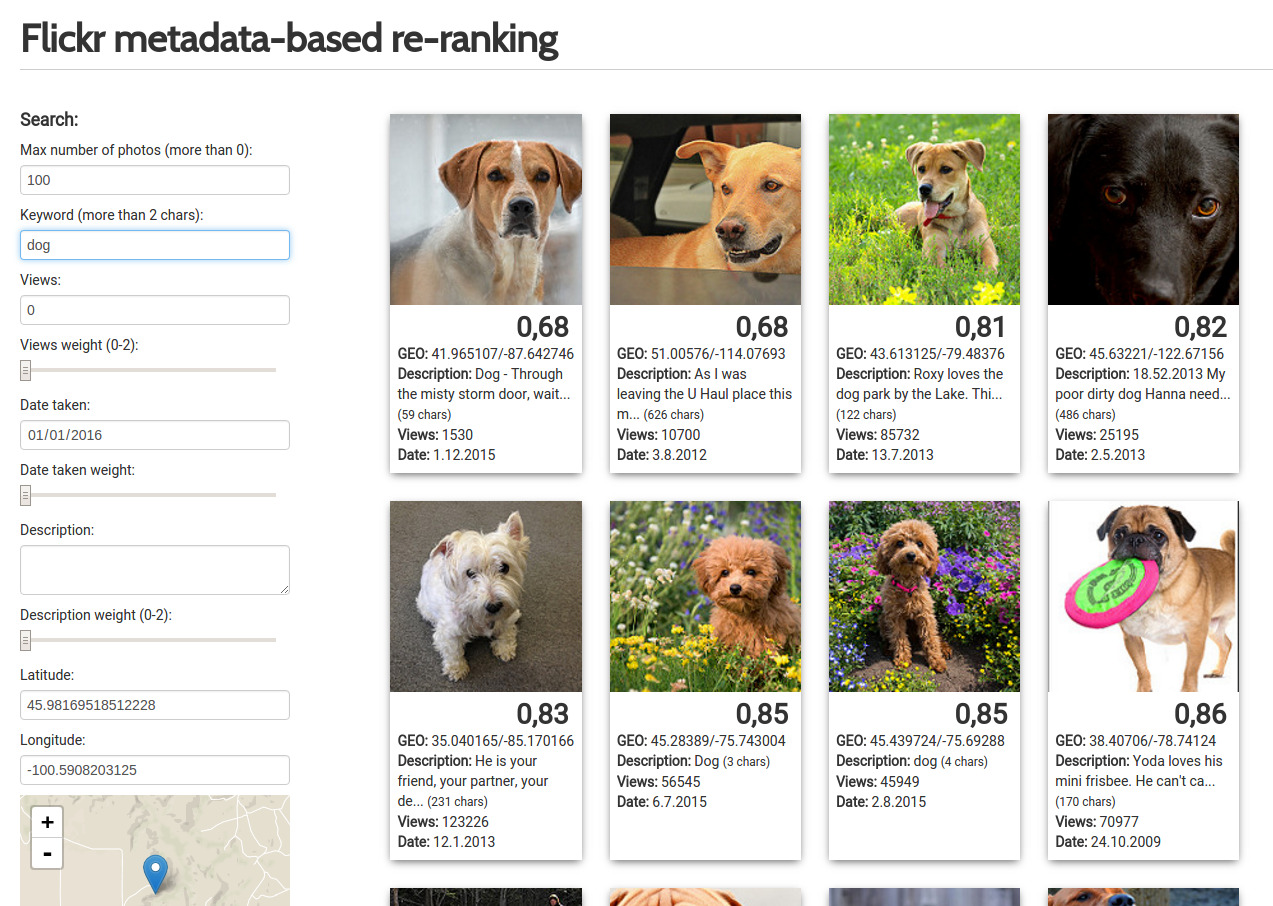
\includegraphics[width=13cm]{pics/layout.png} \caption{Rozvržení aplikace}
\label{fig:layout}
\end{center} \end{figure}

\subsection{Vyhledávání bez/s re-rankingem}
Jako příklad uvádíme vyhledání klíčového slova \texttt{"dakota"}, s tím, že uživatele zajímají fotky ze (Severní/Jižní) Dakoty v USA. Při prostém vyhledávání bez re-rankingu (stahujeme 100 fotek) se sice zobrazí i fotografie z Dakoty, ale jak je vidět na obrázku \ref{fig:dakota_no_geo} kromě nich také fotografie herečky Dakoty Fanning, letadla Douglas DC-3 Dakota a další. Ve výsledku jsou fotografie, které hledáme, v menšině.



\begin{figure}[H] \begin{center}
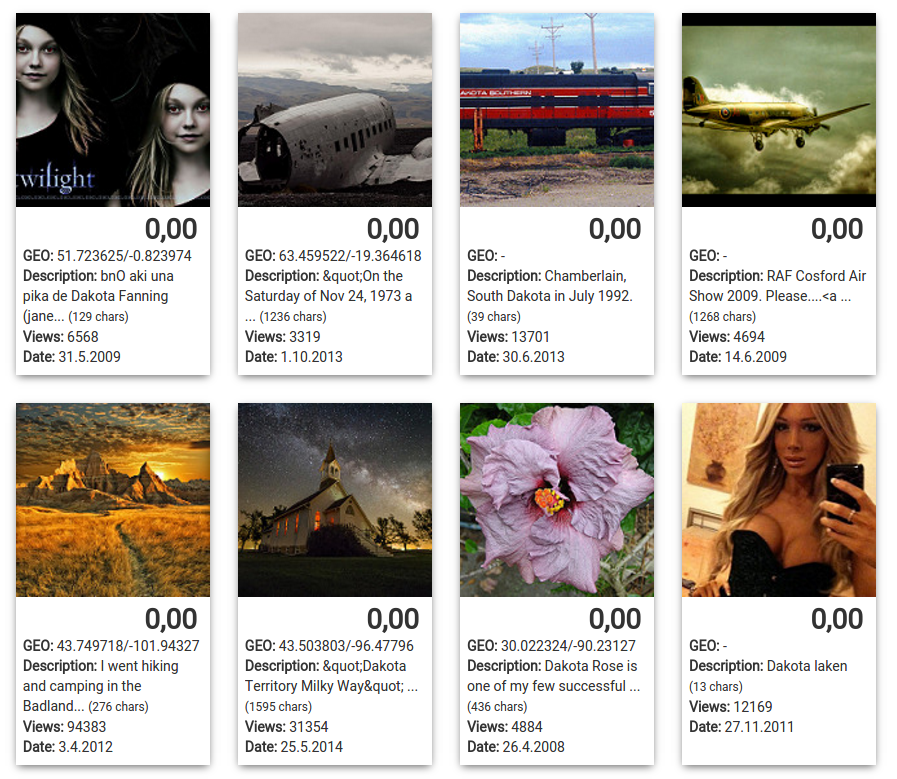
\includegraphics[width=13.5cm]{pics/dakota_no_geo.png} \caption{Vyhledání slova "dakota" bez re-rankingu (prvních 8 výsledků)}
\label{fig:dakota_no_geo}
\end{center} \end{figure}

Při určení požadované polohy fotky (někde na rozmezí Severní a Jižní Dakoty) jsou výsledky diametrálně odlišné -- většina fotografií na prvních pozicích ukazuje přírodu v Dakotě a jinak tematicky zaměřené fotky jsou daleko vzadu (obrázek \ref{fig:dakota_geo}).

\begin{figure} \begin{center}
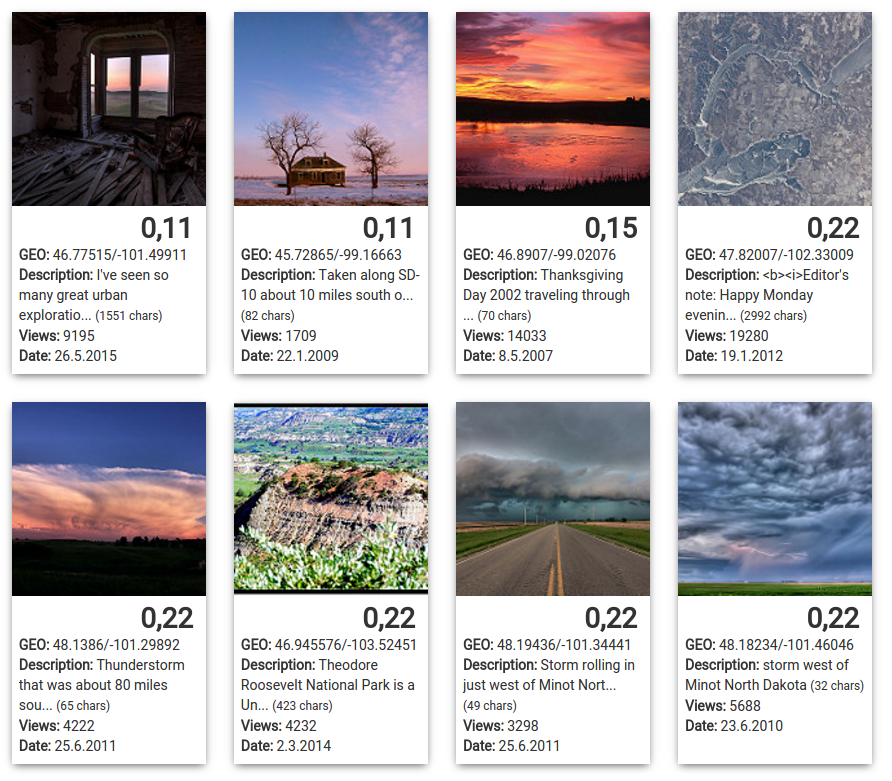
\includegraphics[width=13.5cm]{pics/dakota_geo.png} \caption{Vyhledání slova "dakota" s re-rankingem (prvních 8 výsledků)}
\label{fig:dakota_geo}
\end{center} \end{figure}


\section{Experimentální sekce}
Zde jsme testovali naši verzi programu s návrhem vláknovým zpracováním typu producent (stažení fotek z Flickru) a konzument (reranking). Kdy Reranking zpracovává každou fotku ve vlastním vlákně zajišťující výpočet ranku. Při testování jsme také měnili konfiguraci velikosti stránky pro Flickr API (konfigurační soubor aplikace).

Pro testovací účely ponecháváme na formulářové obrazovce časy zpracování (celkový, stažení, rerakingu, poměr download/ reranking).

Při běžných vstupních hodnotách se stahování fotek (meta dat) z Flickr API se ukázalo jako více omezujícím než jejich reranking. Nastavení velikosti stránky na malou hodnotu (např. pod hodnotu 10 při 150 hledaných fotkách) mělo za následek ještě výraznější zpomalení stahování a proto jsme velikost stránky nastavili 30 s předpokladem počtu stahovaných fotek do 150.

Mluvili jsme o běžných vstupních hodnotách pro reranking. Krajní hodnoty vstupních dat nepředstavují výraznější rozdíl vypočtu ranku až na pole \textit{description}. Zde může uživatel zadat libovolně dlouhý text a čas rankování (funkce pro porovnání dvou řetězců) se tím výrazně prodlužuje. Například při stažení 50 fotek a požití 20 000 znakového textu v \textit{description} se dostáváme na poměr časy pro download/reranking 1/14. Zadání takového textu považuje za spíše teoretické a optimalizace funkce pro porovnání řetězců nepovažujeme za nutnou.

\subsection{Závěr měření:}
Zaměřit se na optimalizace stažení fotek. Zde je možné využít existující princip postupného stahování fotek pomocí stránek a pouze dodělat obalení do samostatných vláken.

\section{Diskuze}
\iffalse
- zadání: "Většina projektů je typu “proof of koncept“, tj. jde o vyzkoušení poznatků
prezentovaných v přednáškách v praxi. Nejde tedy o detailní řešení všech problémů,
které mohou při implementaci nastat – takový projekt by dalece přesahoval rámec
semestrálního projektu. Tato sekce tedy obsahuje rozbor těchto nedostatků a
potenciálním způsobu jejich řešení."
\fi


V projektu zkoušíme řazení podle čtyř typů metadat -- poloha, datum, celé číslo, řetězec. Bylo by samozřejmě možné provádět re-ranking i podle dalších atributů fotografií (např. podle jejich velikosti, poměru stran, \ldots), nicméně principy jsou obdobné. Mohli bychom také např. zohledňovat, v jakém pořadí vrací Flickr fotografie v základním dotazu pomocí klíčového slova.

Naše aplikace také řadí velmi malou podmnožinu fotografií na Flickru -- vždy v reálném čase stáhne daný počet fotografií a porovnává pouze je. Tento nedostatek by se dal vyřešit indexací (části) databáze Flickru do lokální databáze a prací nad těmito daty. Nicméně samotný algoritmus porovnávání by nebylo třeba nijak upravovat -- je nezávislý na množství a zdroji dat.



\section{Závěr}
V rámci semestrální práce jsme se seznámili s principy re-rankingu a navrhli a implementovali webovou aplikaci provádějící re-ranking fotografií ze služby Flickr na základě jejich metadat. V rámci práce na aplikaci jsme naučili využívat některé algoritmy na měření vzdáleností mezi numerickými i nenumerickými hodnotami, např. Levenstheinovu (editační) vzdálenost pro měření vzálenosti mezi dvěma řetězci. Dále jsme si vyzkoušeli, jak dané vzdálenosti kombinovat a normalizovat.

Současně jsme si vyzkoušeli návrh a implementaci vícevláknové aplikace pro konzumaci Flickr API v jazyce Java spolu s jejím frontendem pro uživatelské vstupy a výstupy.  

\renewcommand{\refname}{Literatura}
\bibliographystyle{ieeetr}
{
 \bibliography{refs}
}
\end{document}